% ATENÇÃO - veja com o seu orientador se você vai ter este capítulo e se este vai ter nome!
\chapter{Proposta e metodologia}
\label{cap:proposta}
Neste trabalho é proposto a criação de uma arquitetura que seja capaz de auxiliar na detecção e visualização de vulnerabilidades em redes de computadores. A ideia fundamental é utilizar sensores, com o objetivo de obter a maior quantidade de informações disponíveis a respeito dos dispositivos que serão analisados, criando perfis e utilizando esses perfis para facilitar a administração da rede. Além disso, todas essas informações serão mostradas de maneira gráfica, facilitando para o usuário o entendimento dos resultados obtidos. Para validar a arquitetura proposta será implementada uma ferramenta, na qual será utilizada dois \textit{scanners} para obter informações a respeito da rede analisada, são eles: \gls{OpenVAS} e \gls{Nmap}. As informações obtidas serão utilizadas para auxiliar no gerenciamento e manutenção da rede monitorada. 

A sequência deste capítulo detalha a metodologia utilizada para cumprir o objetivo proposto neste trabalho. Além de explicar detalhadamente a implementação da ferramenta comentada anteriormente.
%---------------------------------------------------%
\section{Metodologia}
A complexidade das redes de computadores aumentou consideravelmente nos últimos anos. De acordo com \citeonline{Gawron:2015:AVD:2799979.2799986} tal complexidade é tão grande que se tornou praticamente impossível gerenciar os riscos de segurança manualmente. Deste modo, ferramentas que auxiliam os administradores de redes na realização de tal gerenciamento tornaram-se necessárias, como por exemplo os \textit{scanners} de vulnerabilidade, \textit{scanners} de rede, entre outras. Porém, os \textit{scanners} tendem a gerar quantidades significativas  de informações, demandando grande tempo dos administradores de redes para analisar e entender tais informações.

Deste modo, a arquitetura proposta deve auxiliar tanto na detecção das vulnerabilidades quanto na visualização dos dados retornados. Tal arquitetura é ilustrada na Figura~\ref{fig:projeto:etapas}.
\begin{figure}[H]
    \centering
    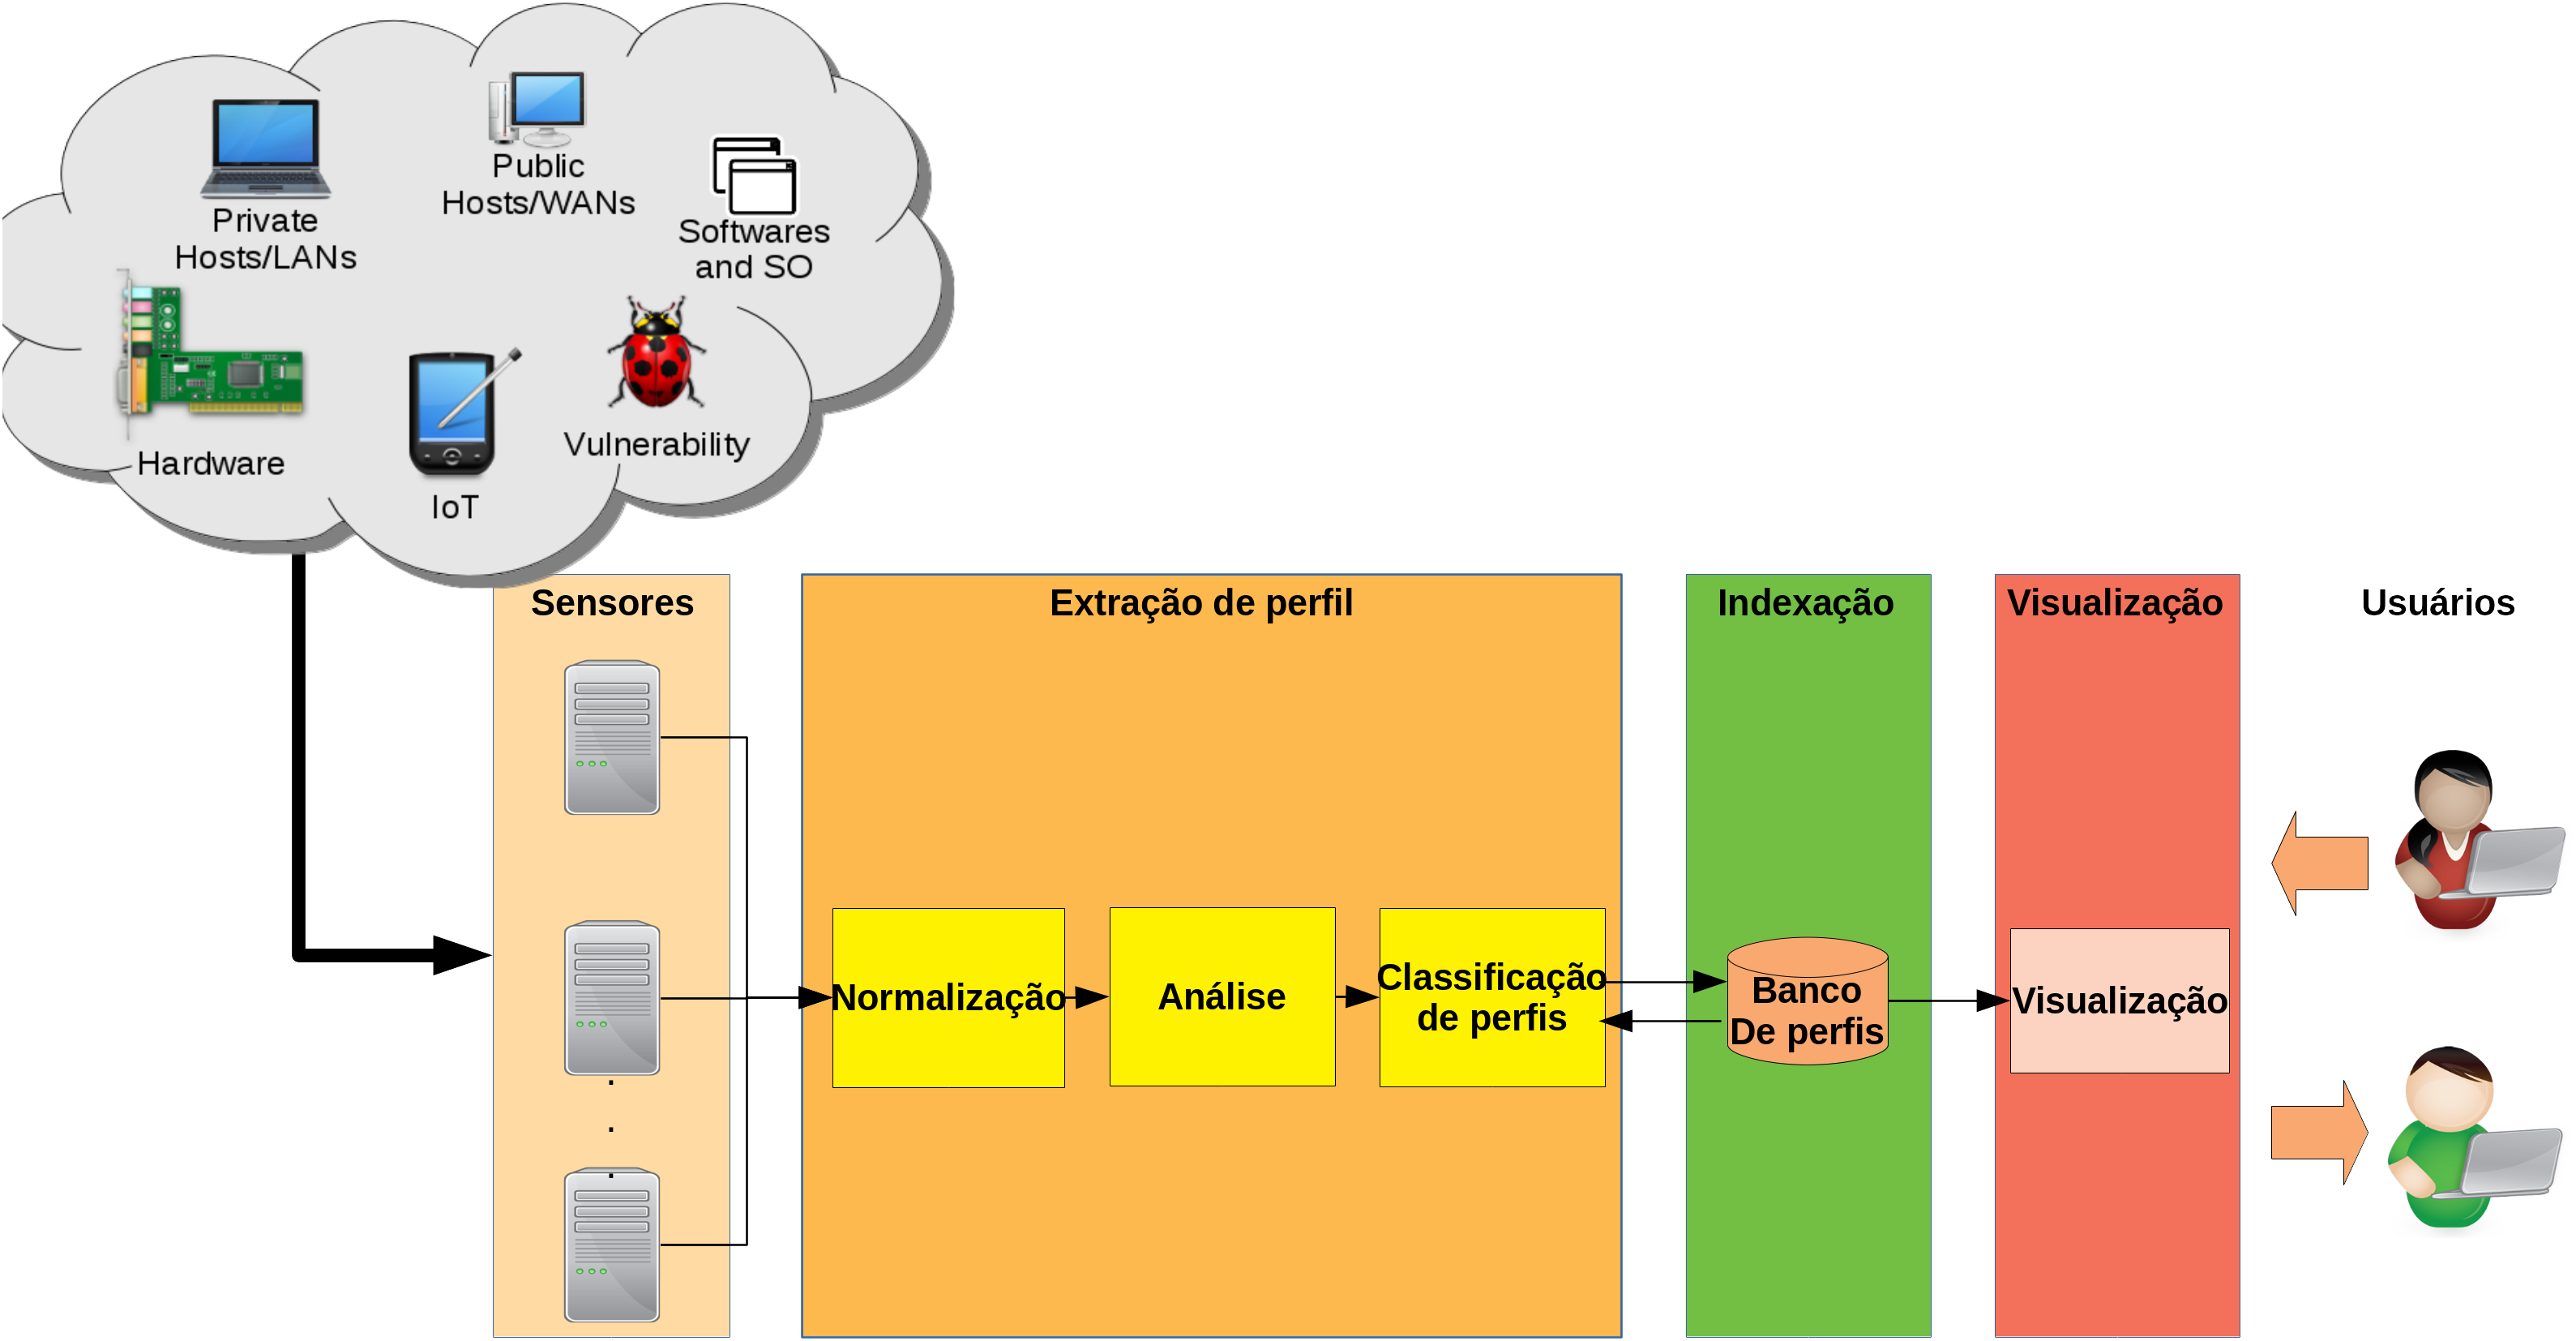
\includegraphics[width=0.90\textwidth]{figuras/tcc.png}
    \caption{Arquitetura proposta.}
    \label{fig:projeto:etapas}
\end{figure}
Conforme a Figura~\ref{fig:projeto:etapas} a arquitetura é composta dos seguintes elementos:
\begin{enumerate}
\item Sensores: Devem coletar o máximo de informações possíveis a respeito dos dispositivos analisados. Vários sensores podem ser utilizados, aumentando a diversidade dos dados coletados.
\item Extração de perfil: Como vários sensores podem ser utilizados na análise dos dispositivos, as informações retornadas devem ser normalizadas, assim, é possível analisar essas informações e extrair características a respeito dos dispositivos analisados, como por exemplo, softwares que estão executando nos dispositivos, sistemas operacionais utilizados, \gls{IP}, entre outras. Essas características serão utilizadas para criação/atualização de perfis, que serão divididos em três grupos, de acordo com a severidade das  vulnerabilidades encontradas nos mesmos, são eles: ``Perfis de alto risco'', ``Perfis de médio risco'', ``Perfis de baixo risco''. Os perfis de alto risco possuem severidades mais graves, portanto possuem uma chance maior de serem invadidos. Os perfis de médio risco, possuem vulnerabilidades de níveis médios, desse modo possuem menos chances de serem invadidos. E os perfis de baixo risco praticamente não possuem vulnerabilidades potenciais para uma invasão. A classificação dos perfis em seus devidos grupos é feita utilizando o valor do \gls{CVSS} de cada vulnerabilidade encontrada no perfil analisado. O \gls{CVSS} é uma métrica utilizada para calcular a severidade de vulnerabilidades. Após a classificação dos perfis os mesmos serão indexados em uma base de dados.
\item Indexação: Os perfis obtidos na extração de perfis serão indexados em um banco de dados, quando uma nova análise da rede é feita as informações nos perfis serão atualizadas e os novos dados serão indexados ao banco juntamente com a sua data. Deste modo será possível manter um histórico dos perfis, tal histórico poderá ser visualizado pelos usuários, para verificar se novas vulnerabilidades foram encontradas desde a última varredura realizada. Essas informações serão utilizadas para gerar visualizações a respeito dos ambientes analisados, auxiliando os usuários da ferramenta na administração da rede monitorada.
\item Visualização: Os usuários do sistemas poderão observar os dados obtidos através de uma interface, visando melhor entendimento das informações coletadas, como por exemplo, obter uma visão geral da topologia da rede analisada, visualizar as informações sobre os dispositivos, entre outras.
\end{enumerate}


Para validar a arquitetura proposta uma ferramenta será implementada. A ferramenta utilizará dois sensores, um para obter informações vindas do \textit{scanner} de rede \gls{Nmap} e outro para capturar as informações do \textit{scanner} de vulnerabilidade \gls{OpenVAS}. O \gls{Nmap} será utilizado para obter as portas de redes abertas, as aplicações que estão executando nessas portas, os sistemas operacionais e o \gls{MAC} dos dispositivos. O \gls{MAC} é um valor único, associado à interface de comunicação utilizada pelo dispositivo para se conectar a rede. Tal valor será utilizado como uma identificação única dos dispositivos analisados. O outro sensor será o \gls{OpenVAS} no qual será utilizado para obter as vulnerabilidades existentes nos dispositivos. Essas informações serão retornadas em um arquivo \gls{XML}.

O arquivo \gls{XML} gerado anteriormente será analisado, e a partir das informações encontradas neste arquivo serão gerados os perfis dos dispositivos. Um \textit{script} implementado na linguagem de programação Python\footnote{\url{https://www.python.org/}} será utilizado para analisar o arquivo \gls{XML} e criar os perfis dos dispositivos. O \textit{script} percorre as \textit{tags} \gls{XML} e coleta as informações contidas nas mesmas. As vulnerabilidades retornadas pelo \gls{OpenVAS} marcadas como ``\textit{log}'' não serão utilizadas, pois são informações semelhantes às retornadas pelo \gls{Nmap}.  O \textit{script} retorna as informações filtradas no formato \gls{JSON}. Tal formato foi escolhido devido a sua simplicidade e a facilidade de integração com o motor e busca Elasticsearch, que será utilizado neste trabalho. O código a seguir apresenta um exemplo de arquivo obtido no término da execução do \textit{script}.


%\item Obter informações dos sistemas: Sensores devem obter o máximo de informações possíveis a respeito os sistemas analisados, vários sensores podem ser utilizados nesta etapa da arquitetura, como por exemplo, \textit{scanners} de rede, \textit{scanners} de vulnerabilidades, ferramentas para análise do fluxo de dados na rede, entre outras, depois de obter as informações, as mesmas devem ser normalizadas, para que se possa extrair características que serão utilizadas para ; 
%\item Extração de perfis: Toda informação obtida na etapa anterior será normalizada, para que se consiga analisar essas informações e extrair características, que serão usadas para montar um perfil para cada sistema analisado. Os perfis podem ser divididos em dois grupos, são eles: ``Perfis vulneraveis'' e ``Perfis normais''. Os ``Perfis vulneraveis'' são informações sobre sistemas que de algum modo já sofreram intrusão ou outro tipo de ataque bem sucedido. O sistema Horus será responsável por ceder os sistemas que já sofreram ataques(>>melhorar). Os ``Perfis normais'' possuem informações dos sistemas analisados pelo sensores que não tenham sidos explorados. Estes perfis serão utilizados para gerar visualizações sobre o ambiente analisado, realizar comparações de similaridade de perfis, entre outras funções;
%\item Indexação: Os perfis obtidos na etapa anterior serão indexados em um motor de busca, onde serão feitas as comparações de similaridade entre perfis do grupo ``Perfis vulneraveis'' com perfis do grupo ``Perfis normais'', além disso, as informações indexadas serão utilizadas para gerarem uma visualização mais detalhada do ambiente analisado; 
%\item Comparação de perfis: Comparar perfis de dispositivos analisados com os perfis vulneráveis;
%\item Visualização de dados: Mostrar os dados obtidos para o usuário.
%As etapas da arquitetura serão explicadas detalhadamente a seguir.


%O arquivo \gls{XML} gerado na etapa 1 precisa ser filtrado e organizado de maneira que seja montado um perfil para cada dispositivo analisado. Portanto, na etapa 2, o \gls{XML} é filtrado visando diminuir a quantidade dos dados retornados pelos \textit{scanners}, tal filtragem é realizada utilizando um \textit{script}, implementado na linguagem de programação python\footnote{\url{https://www.python.org/}}. O \textit{script} percorre as \textit{tags} \gls{XML} e coleta as informações contidas nas mesmas. As vulnerabilidades retornadas do \gls{OpenVAS} marcadas como ``\textit{log}'' serão desconsideradas pois são informações semelhantes as retornadas pelo \gls{Nmap}.  O \textit{script} retorna as informações filtradas no formato \gls{JSON}, tal formato foi escolhido devido a sua simplicidade e a facilidade de integração com o banco de dados não-relacional ElasticSearch, que armazena os dados no formato  \gls{JSON}. A Figura~\ref{fig:formato:json} apresenta o arquivo obtido após a filtragem das informações.
\begin{lstlisting}[style=json, label=arquivo:json:output, caption={Exemplo de arquivo \gls{JSON} gerado a partir das informações.}, basicstyle=\scalefont{0.6}]
{
      "MAC":"90:2B:34:3C:7C:97",
      "OS":"Linux 3.2 - 4.6",
      "Ports":{
         "22":"OpenSSH 7.2p2 Ubuntu 4ubuntu2.1 (Ubuntu Linux; protocol 2.0)",
         "80":"Apache httpd 2.2.22 ((Ubuntu))",
         "443":"lighttpd 1.4.13"
      },
      "Hardware":"Giga-byte Technology",
      "vuls":[
         {
            "Threat":"High",
            "IP":"172.16.2.136",
            "CVSS":"7.1",
            "Protocol":"tcp",
            "Port":"80",
            "OID":"1.3.6.1.4.1.25623.1.0.800827",
            "Name":"Apache 'mod_proxy_http.c' Denial Of Service Vulnerability",
            "Impact":"Successful exploitation will allow remote attackers to cause Denial of Service to the legitimate user by CPU consumption. Impact Level: Application",
            "CVE":"CVE-2009-1890",
            "References":"http://secunia.com/advisories/35691 http://www.vupen.com/english/advisories/2009/1773",
            "Date":"2017-09-19T01:17:47Z"
         }]
}
\end{lstlisting}

O \gls{JSON} obtido para a criação dos perfis no banco contém os seguintes campos:
\begin{itemize}
    \item \gls{MAC}: Valor único, utilizado para identificar um dispositivo de rede perante aos outros;
    \item \gls{OS}: Sistema operacional executando no dispositivo;
    \item \textit{Ports} (Portas): Portas de rede encontradas abertas;
    \item Hardware: Hardware do dispositivo;
\end{itemize}
Além dessas informações, também existe um vetor de vulnerabilidades, com os seguintes campos:
\begin{itemize}
    \item \textit{Threat} (ameaça): O nível de ameaça que tal vulnerabilidade representa para o sistema em qual foi detectada, os \textit{scanners} testados no presente trabalho possuem 4 níveis de ameaças,  alto(\textit{high}) , médio (\textit{medium}),  baixo (\textit{low}) e informações  (\textit{logs}), esses níveis são determinados utilizando a pontuação obtida durante o cálculo do \gls{CVSS}.  Os \textit{logs} não são considerados ameaças, são informações que o \textit{scanner} conseguiu adquirir do sistema alvo (sistema operacional, versões de aplicativos instalados, entre outras);
    \item \gls{CVSS}: Uma métrica padrão para calcular o nível de severidade das vulnerabilidades. O cálculo é feito levando em consideração a facilidade para explorar a vulnerabilidade e o impacto da exploração. Após o cálculo, uma pontuação é atribuída a tal vulnerabilidade, podendo ir de 0 até 10, onde 10 é considerado severidade máxima \cite{cvss};
    \item \textit{Protocol} (protocolo): Protocolo de comunicação de rede utilizado quando a vulnerabilidade foi detectada;
    \item \textit{Port} (porta): Porta de rede em qual a vulnerabilidade foi detectada;
    \item OID: Identificador único de vulnerabilidades dentro da base de dados do \gls{OpenVAS};
    \item \textit{Name} (nome): Nome da vulnerabilidade;
    \item \textit{Impact} (impacto): Impacto para o sistema caso ocorra a exploração da vulnerabilidade;
    \item \gls{CVE}: Uma base de dados internacional contendo características de vulnerabilidades descobertas\footnote{\url{https://cve.mitre.org/}};
    \item \textit{References} (referências): Informações a respeito das vulnerabilidades;
    \item \textit{Date} (data): A data exata contendo dia, mês, ano, horas, minutos e segundos na qual a vulnerabilidade foi detectada.
\end{itemize}

O \gls{JSON} será persistido em um banco de dados. Para implementar este trabalho foi escolhido o motor de busca Elasticsearch. Para a visualização dos dados será utilizado o \textit{plugin} Kibana. A partir dos dados contidos no Elasticsearch, através de uma interface web, o usuário é capaz de analisar todas as informações a partir de gráficos dos mais variados estilos, como por exemplo, gráfico de barras, gráficos de linhas, entre outros.


Deste modo, a ferramenta é capaz de simplificar a análise de dos dados obtidos através dos \textit{scanners} utilizados, auxiliando os usuários na detecção e visualização de vulnerabilidades, facilitando também no gerenciamento de redes de computadores.


%--------------------------------------------------%
\section{Cronograma de Atividades}

Nesta seção são apresentadas as atividades a serem desenvolvidas para a execução da proposta. O cronograma de realização das tarefas é apresentado na Tabela~\ref{tab:cronograma}.


Os seguintes itens fazem parte do cronograma:

\begin{enumerate}
\item \textbf{Estudo da ferramenta ElasticSearch.}
\item \textbf{Persistência dos dados no banco.}
\item \textbf{Implementação da Ferramenta proposta.}
\item \textbf{Estudo da ferramenta Kibana.}
\item \textbf{Realização dos experimentos utilizando a ferramenta proposta.}
\item \textbf{Teste e análise dos resultados obtidos.}
\item \textbf{Escrita do TCC2}
\item \textbf{Entrega do TCC 2.}
\item \textbf{Apresentação do TCC 2.}
\end{enumerate}




% Please add the following required packages to your document preamble:
% \usepackage{multirow}
% Please add the following required packages to your document preamble:
% \usepackage{multirow}
\begin{table}[H]
\renewcommand{\arraystretch}{1.3}
\centering
\caption{Cronograma das Atividades}
\label{tab:cronograma}
\scalefont{0.9}
\begin{tabular}{|l|l|l|l|l|l|l|l|l|}
\hline
\multicolumn{1}{|c|}{\multirow{2}{*}{\textbf{Atividade}}} & \multicolumn{6}{c|}{\textbf{2018}}         \\ \cline{2-7} 
\multicolumn{1}{|c|}{}                           & \textbf{Jan} & \textbf{Fev} & \textbf{Mar} & \textbf{Abr} & \textbf{Mai} & \textbf{Jun} \\ \hline
\textbf{1}                                                & X   &     &     &     &     &     \\ \hline
\textbf{2}                                                &  X   &    &     &     &     &     \\ \hline
\textbf{3}                                                &  X   &  X   & X    &    X& X    &     \\ \hline
\textbf{4}                                                &     &    X &     &     &     &     \\ \hline
\textbf{5}                                                &     &     &     X&  X   &     &     \\ \hline
\textbf{6}                                                &     &     &     &    X &    X &     \\ \hline
\textbf{7}                                                &   X  &   X  &X     &   X  & X    & X    \\ \hline
\textbf{8}                                                &     &     &     &     &     &     X\\ \hline
\textbf{9}                                                &     &     &     &     &     &     X\\ \hline
\end{tabular}
\end{table}
